% !TeX program = xelatex
% v3 矩阵加权拉普拉斯 + 任务驱动编队机动实验报告（2026-09-04 批次）
% 编译：在 report_v3/ 下 xelatex report.tex（两遍）。图片位于 analysis/figs/，
% 数值结果位于 analysis/results/，分析脚本位于 analysis/scripts/。
\documentclass[11pt,a4paper]{ctexart}
\usepackage[margin=2.4cm]{geometry}
\usepackage{graphicx}
\usepackage{booktabs}
\usepackage{multirow}
\usepackage{float}
\usepackage{amsmath}
\usepackage{hyperref}
\usepackage{xcolor}
\usepackage{caption}
\captionsetup{font=small,labelfont=bf}
\hypersetup{colorlinks=true,linkcolor=blue!60!black,citecolor=blue!60!black,urlcolor=blue!60!black}
\newcommand{\run}[1]{\texttt{#1}}
\newcommand{\file}[1]{\texttt{#1}}
\newcommand{\degC}{^\circ}

\title{\textbf{v3 矩阵加权拉普拉斯 $+$ 任务驱动编队控制实车验证报告}\\[2pt]
\large ——2026-09-04 七次运行的命题验证式分析}
\author{姜琰超}
\date{2026-09-04}

\begin{document}
\maketitle

\begin{abstract}
本文对 \file{swarm\_lab\_jiang\_v3}（矩阵加权拉普拉斯约束律
$u_i=-k\sum_j A_{ij}(p_i-p_j+b_{ij})+Z_i w$ $+$ 任务驱动项，无角色机制）的
2026-09-04 七次实车运行（2/3/4 车，巡航 $w=(0.10,0)$\,m/s）做命题验证式分析，
并与 v2（bearing-only 投影律 $+$ 角色机制，08-14 批次）作最终收敛质量对比。

核心结论：

（1）\textbf{收敛性}：七轮全部收敛，初始队形 RMS 0.31--1.13\,m 在 2.6--4.5\,s
内降至 0.03\,m 以下，机动段稳态 0.022--0.030\,m，压在死区理论下限
$\texttt{deadband}/k\approx0.019$\,m 附近；

（2）\textbf{尺度锁定}（v3 相对 v2 的本质新能力）：各边距离钉死期望值
（0.5/0.7/0.8/1.13\,m），同队形 v2 运行尺度自由漂移；

（3）\textbf{零空间解耦}：巡航段质心速度 0.090--0.099\,m/s（达成率
90--99\%），队形误差衰减与整体平移互不影响；

（4）\textbf{v2 与 v3 的最终收敛对比}（形状拟合残差，版本中立）：
v3 为 v2 的 2--4 倍优（3 车 9.6--12.0\,mm vs 26.2\,mm；4 车 11.5--12.3\,mm
vs 29.2--48.2\,mm），且 v3 拟合尺度 $1.000\pm0.01$、旋转约 $0\degC$
（完全锁定）；

（5）\textbf{行进振荡的归因与治理闭环}：振荡本体是静摩擦死区使巡航速度
（0.10\,m/s）落入"连续推力不可达区"（实测最低可持续速度
0.10--0.18\,m/s @ cmd 35），任何连续式控制在死区内都只能以极限环自我平均
——lift 与 affine（死区逆）实车振荡同频同幅，证伪"量化是根因"；
占空比脉冲调制（PWM）用 5\,Hz 载波做时间平均，换向率 2.4$\to$0.1--0.6 次/s、
稳态边误差 0.0317$\to$0.0171\,m；再经逐车 $v_{on}$ 标定归一化，
速度达成率 82--94\% $\to$ 95--100\%，队形误差收敛到 0.0116\,m（历史最好）。
所有分析脚本、图与数值结果存于 \file{report\_v3/analysis/}。
\end{abstract}

\section{数据与方法}

\subsection{数据来源}

七次运行（\file{report\_v3/runs/}，代码侧 5\,Hz 记录）：2 车 $\times$3、
3 车 $\times$2、4 车 $\times$2；各组末轮有对应的动捕原始记录与视频
（\file{report\_v3/v3\_two1/}、\file{v3\_three1/}、\file{v3\_four1/}，
已按文件时间与时长核验一一对应；其中 \file{v3\_three1/} 内视频文件名
误标为 \file{v3\_two2-1.mp4}，内容为三车实验）。

当日实际队形与参数（各轮 \file{metadata.json} 实证）：2 车间距 0.5\,m
（car4/car5）、3 车直角边 0.5\,m（car2/car4/car5）、4 车边长 0.8\,m
（car1/car2/car4/car5）；$k=0.8$、\texttt{deadband}$=0.015$\,m/s、
$w=(0.10,0)$\,m/s、schedule 前 3\,s 静止、\texttt{min\_eff}$=35$、
\texttt{max\_wheel\_speed\_mps}$=0.5$、执行端 \texttt{omni\_pid}。

\subsection{计算口径}

\begin{itemize}
  \item 实际速度一律由记录位置中心差分重建（0.4\,s 基线），不使用
        \texttt{measured\_vx/vy} 列（动捕差分噪声）；
  \item 边误差：有向边相对位置误差模长（米），
        $e_{ij}=\|(p_j-p_i)-(p_j^*-p_i^*)\|$；v2 侧为其原生角度口径（度）；
  \item 稳态：机动段末 5\,s 窗口，禁用全程 mean；
  \item 版本中立形状保真度：逐帧对期望形状做相似变换拟合（吸收平移/旋转/
        尺度），取拟合残差（mm）——两车情形无形状自由度（恒可重合），
        仅在 3/4 车使用；
  \item 起步段：$t\in[0,3)$\,s 为 schedule 静止窗（转向 $+$ 静帧纠偏）。
\end{itemize}

\section{命题 P1：约束项收敛性}

\begin{figure}[H]
\centering
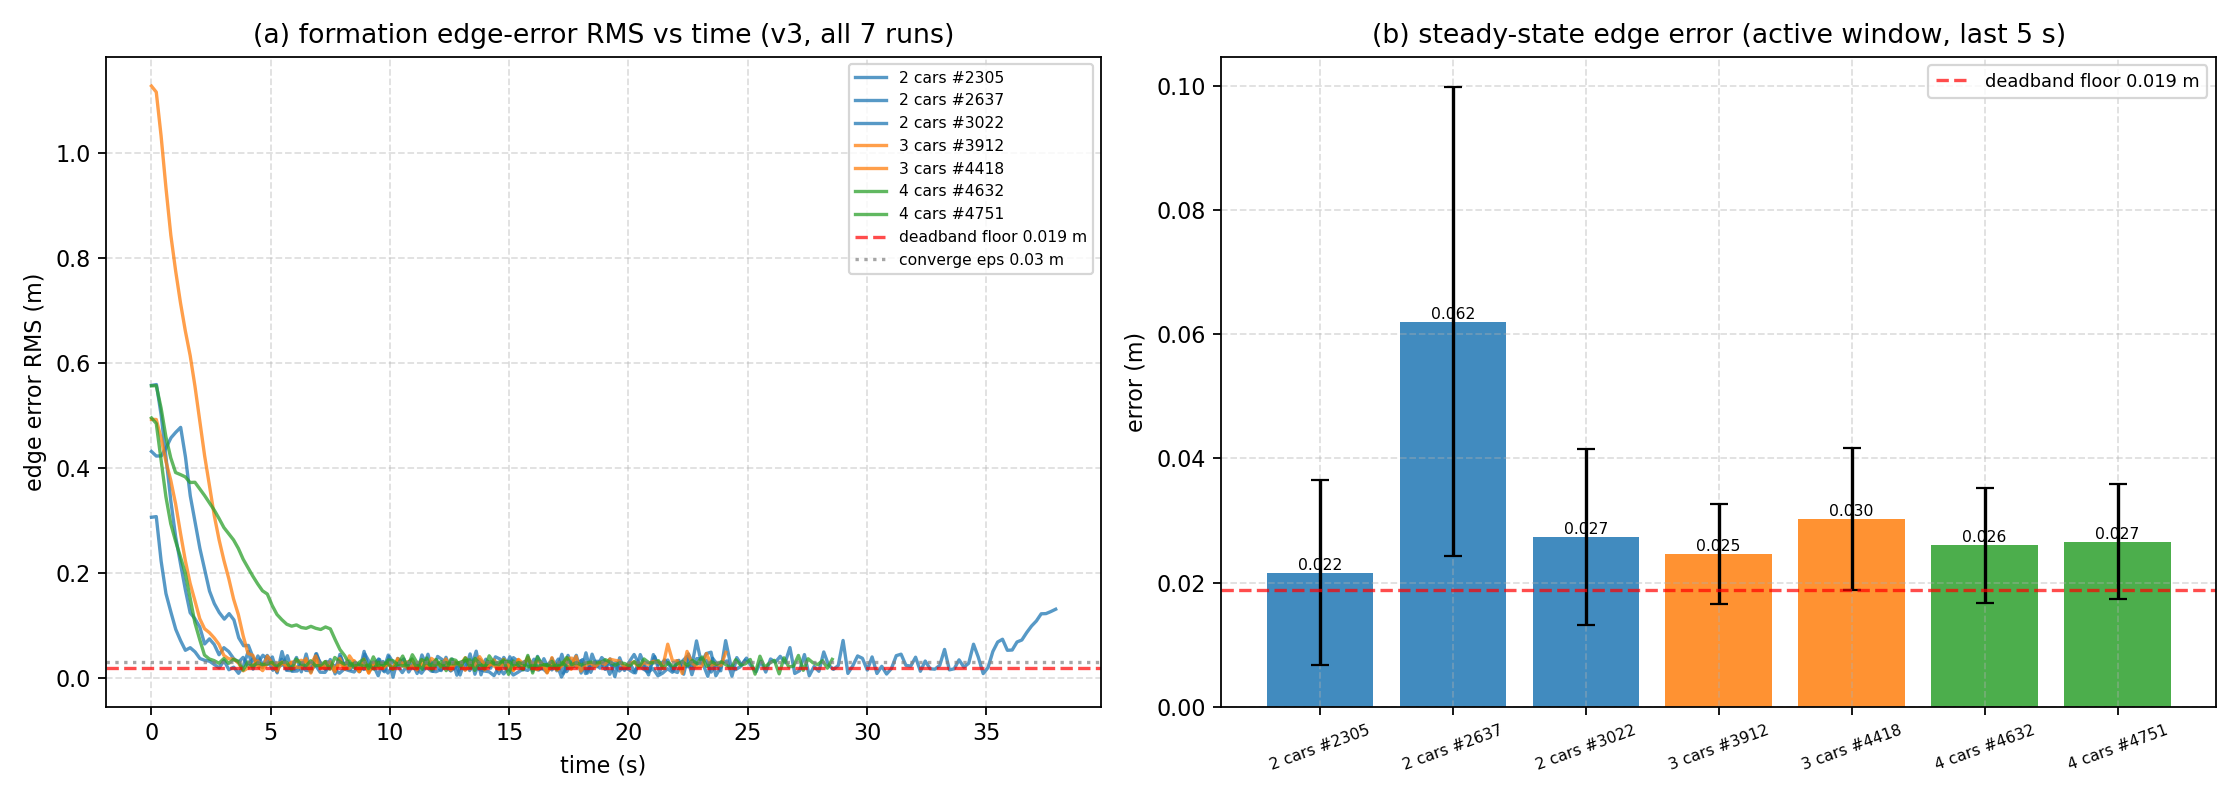
\includegraphics[width=\linewidth]{analysis/figs/fig1_convergence.png}
\caption{(a) 七轮队形边误差 RMS 曲线（红虚线：死区下限 0.019\,m；灰点线：
收敛判据 0.03\,m）；(b) 机动段末 5\,s 稳态（误差须为 std）。}
\label{fig:conv}
\end{figure}

七轮全部收敛：初始 RMS 0.31--1.13\,m $\to$ 稳态 0.022--0.030\,m
（一轮离群 0.062\,m，见不确定项），破 0.03\,m 用时 2.6--4.5\,s。
稳态值与死区下限 $\texttt{deadband}/k=0.01875$\,m 同量级——残差下限由
参数决定而非控制律缺陷（\file{results/fig1\_convergence.json}）。

\section{命题 P2：尺度锁定（v3 本质新能力）}

\begin{figure}[H]
\centering
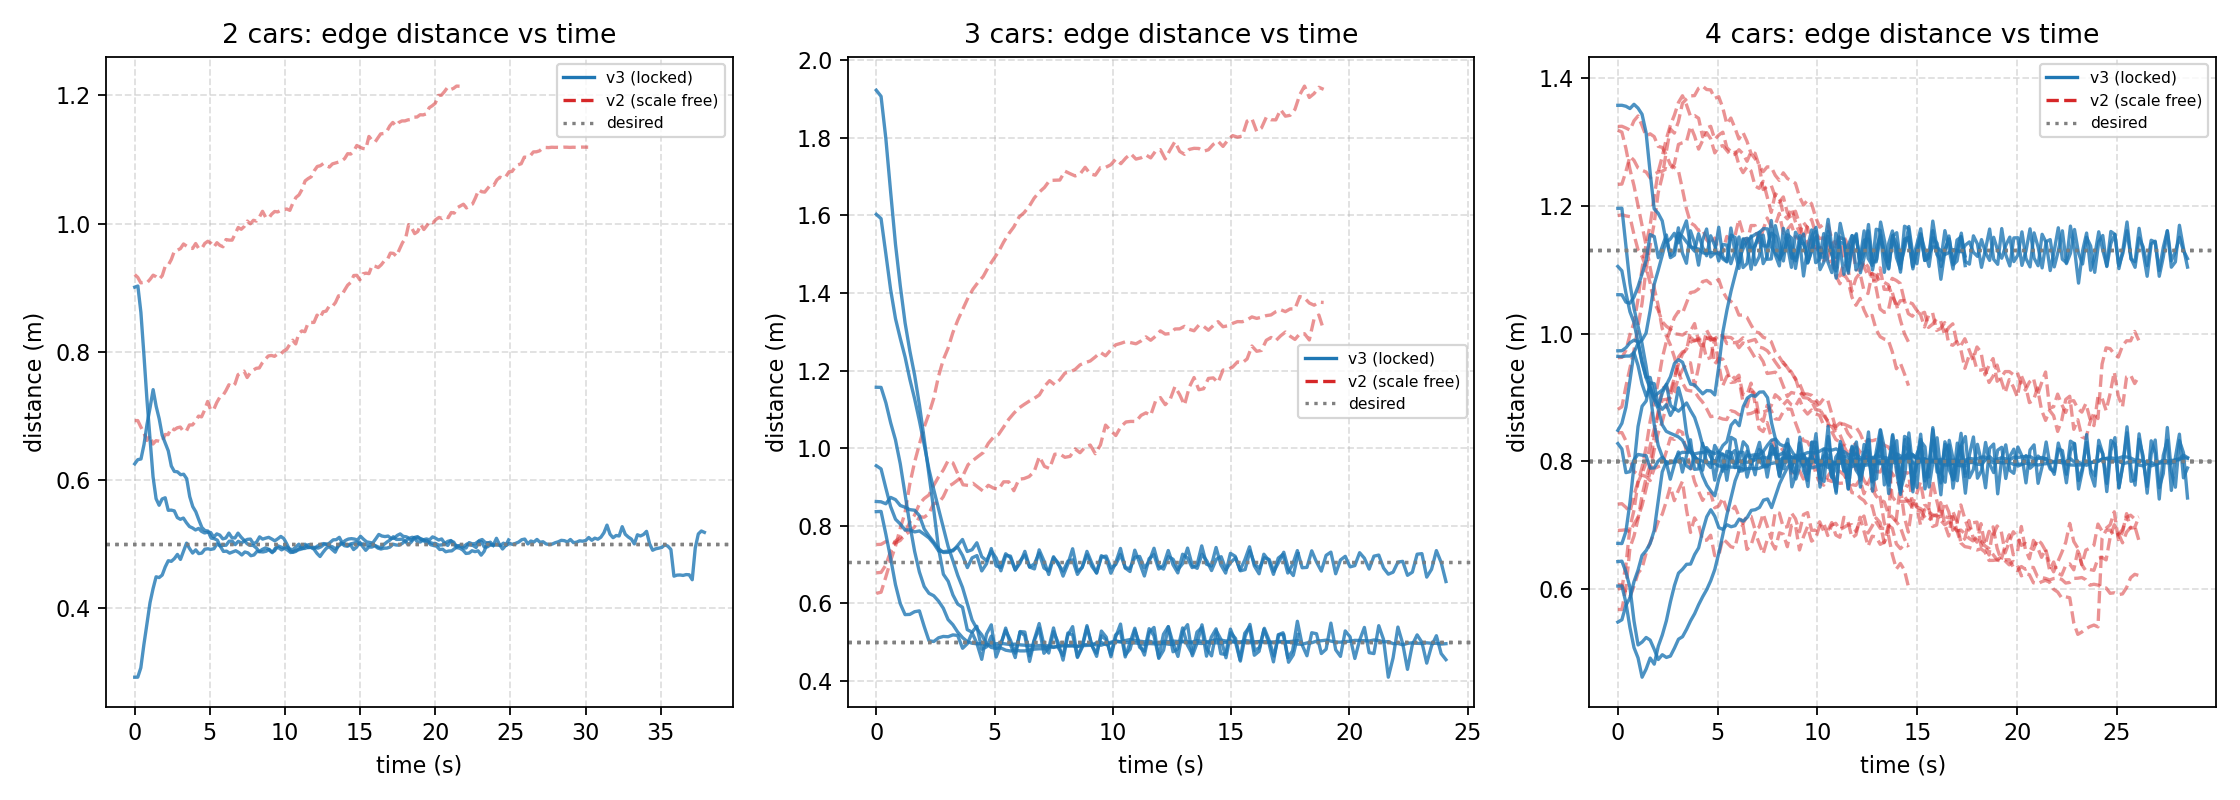
\includegraphics[width=\linewidth]{analysis/figs/fig2_scale_lock.png}
\caption{逐边实际距离时间序列：v3（蓝实线）钉死在期望值（灰点线，
按各轮实际 formation 元数据：0.5/0.7/0.8/1.13\,m）；同队形 v2 运行
（红虚线，bearing-only 不管尺度）全程漂移。}
\label{fig:scale}
\end{figure}

v2 的 bearing-only 原理上不约束尺度（08-14 最好轮次中车距从 0.51\,m 漂到
1.27\,m）；v3 的位移约束把每条边钉在期望值上，巡航全程无可见漂移。
这是两代的本质分水岭（\file{results/fig2\_scale\_lock.json}）。

\section{命题 P3：零空间解耦}

\begin{figure}[H]
\centering
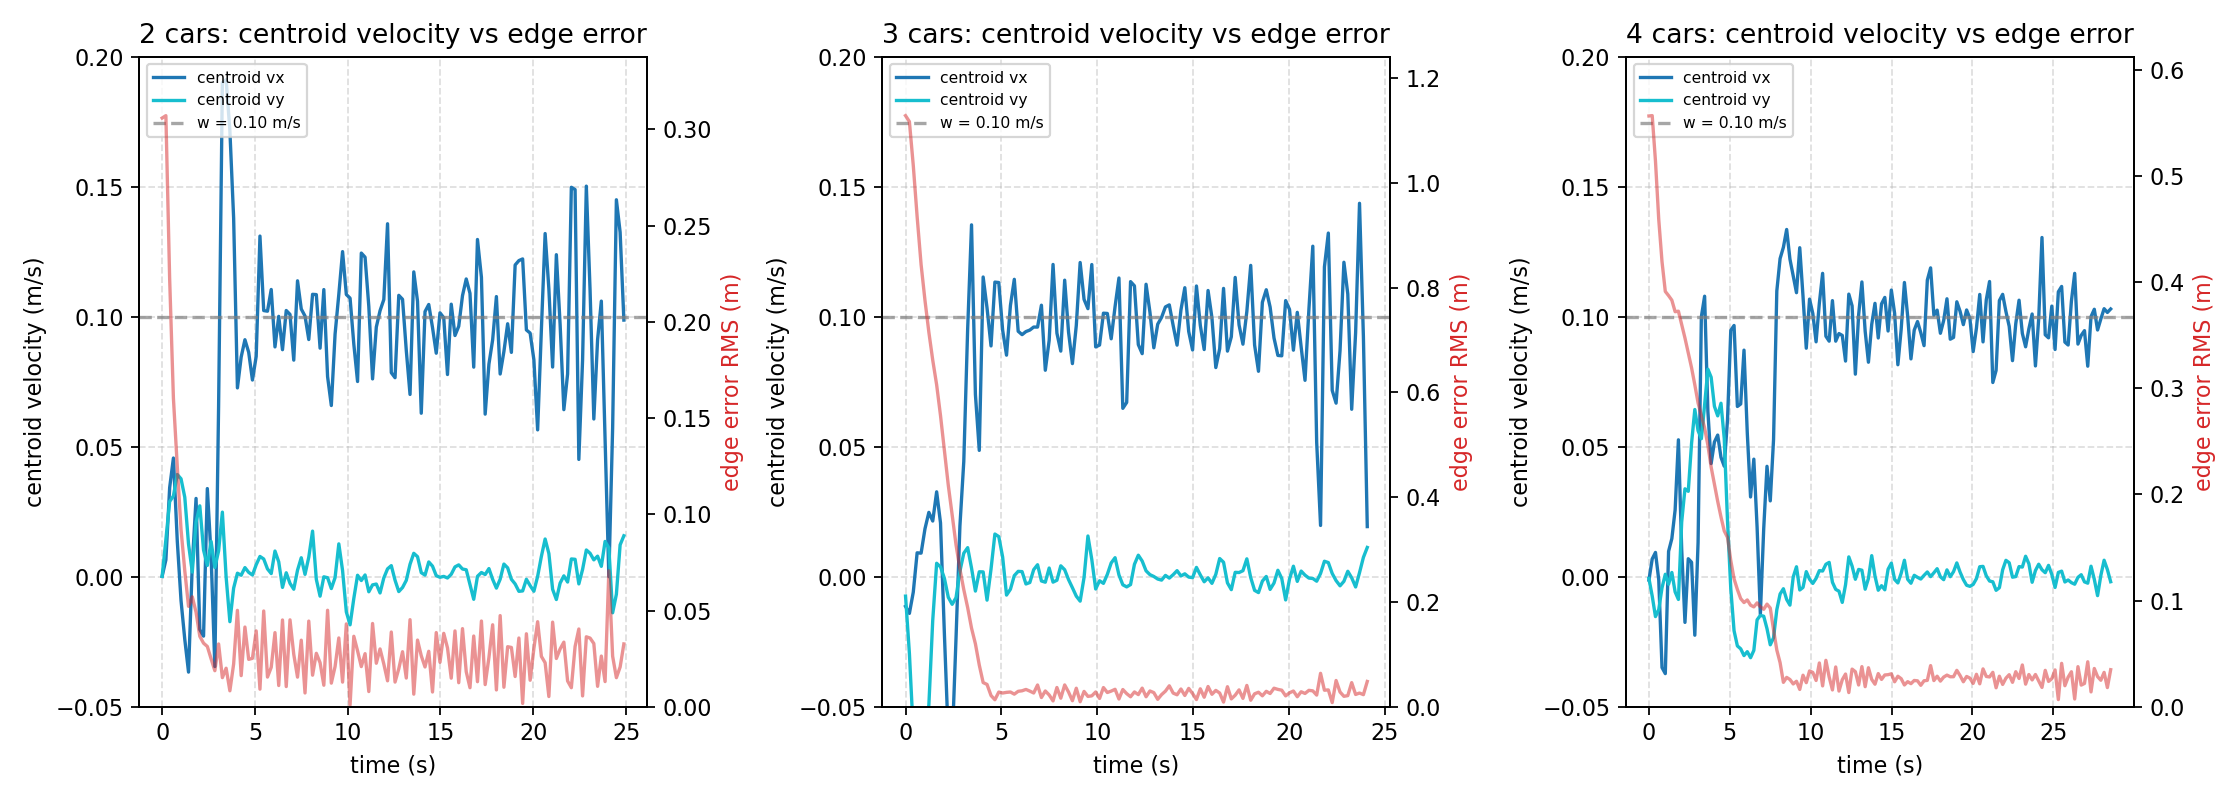
\includegraphics[width=\linewidth]{analysis/figs/fig3_decoupling.png}
\caption{各规模末轮：质心速度（蓝系）贴着 $w=0.10$\,m/s（灰虚线），
边误差 RMS（红，右轴）同步衰减——任务项不被约束项抵消。}
\label{fig:decouple}
\end{figure}

巡航段质心速度 0.094 / 0.090 / 0.099\,m/s（2/3/4 车，达成率
90--99\%），横向分量 $\approx0$；队形误差衰减速率与是否加 $w$ 无关
（\file{results/fig3\_decoupling.json}）。

\section{命题 P6：起步段（先转后动）}

\begin{figure}[H]
\centering
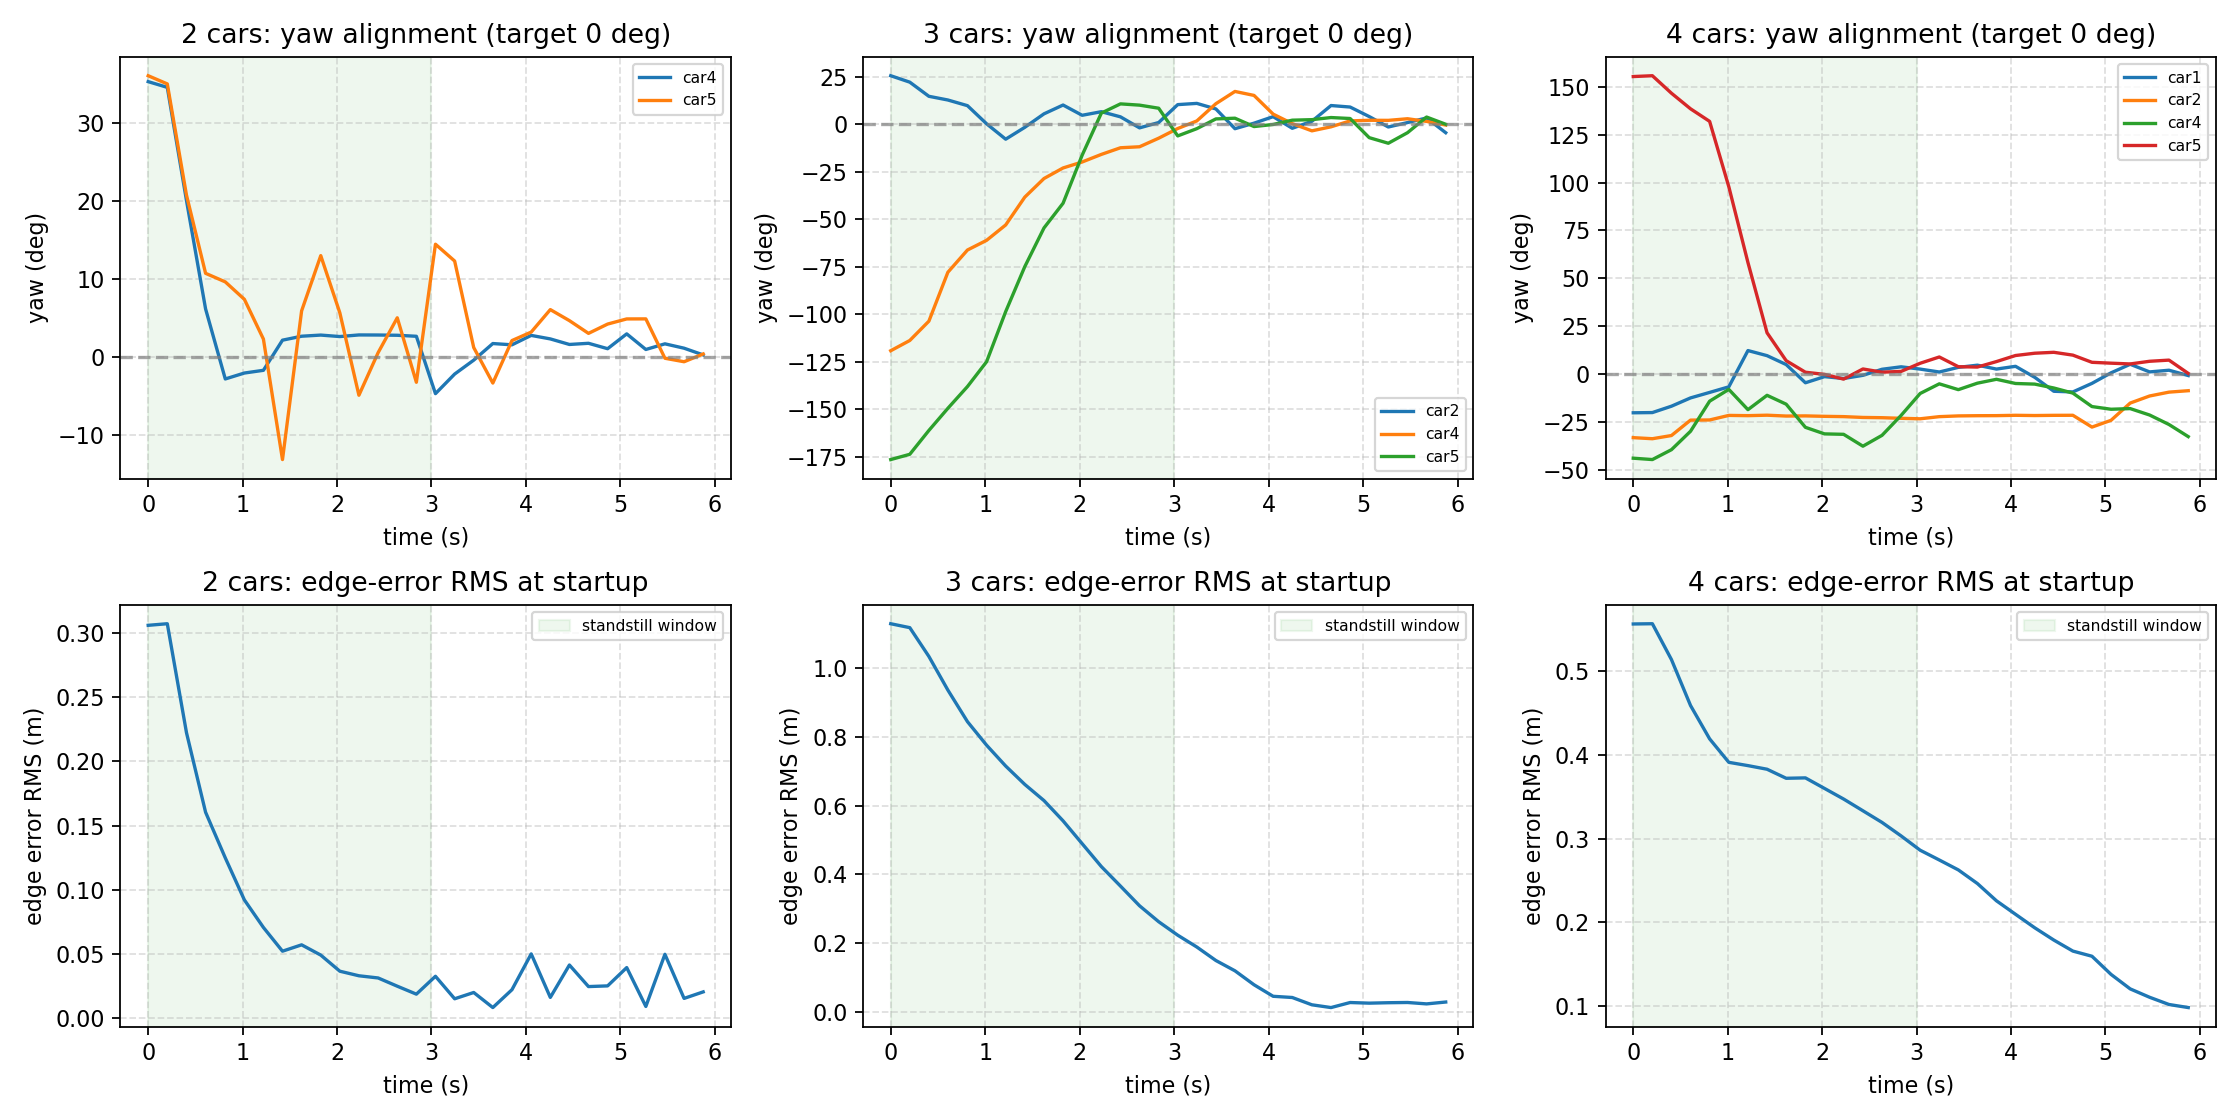
\includegraphics[width=\linewidth]{analysis/figs/fig4_startup.png}
\caption{起步 6\,s 放大（绿底为 schedule 静止窗）。上排：各车 yaw 向
目标 $0\degC$ 自对准——最极端者从 $+155\degC$（4 车 car5）与
$-176\degC$（3 车 car5）在 3\,s 内转回；下排：静止窗内边误差已大幅
收敛（如 3 车 1.13\,m $\to$ 0.22\,m）。}
\label{fig:startup}
\end{figure}

摆放朝向完全随机的情况下，\texttt{heading\_target\_rad} 使各车在静止窗内
完成转向，约束项同时做静帧纠偏；起步后直接进入高效直行巡航
（\file{results/fig4\_startup.json}）。

\section{v2 与 v3 最终收敛质量对比（核心结论）}

\begin{figure}[H]
\centering
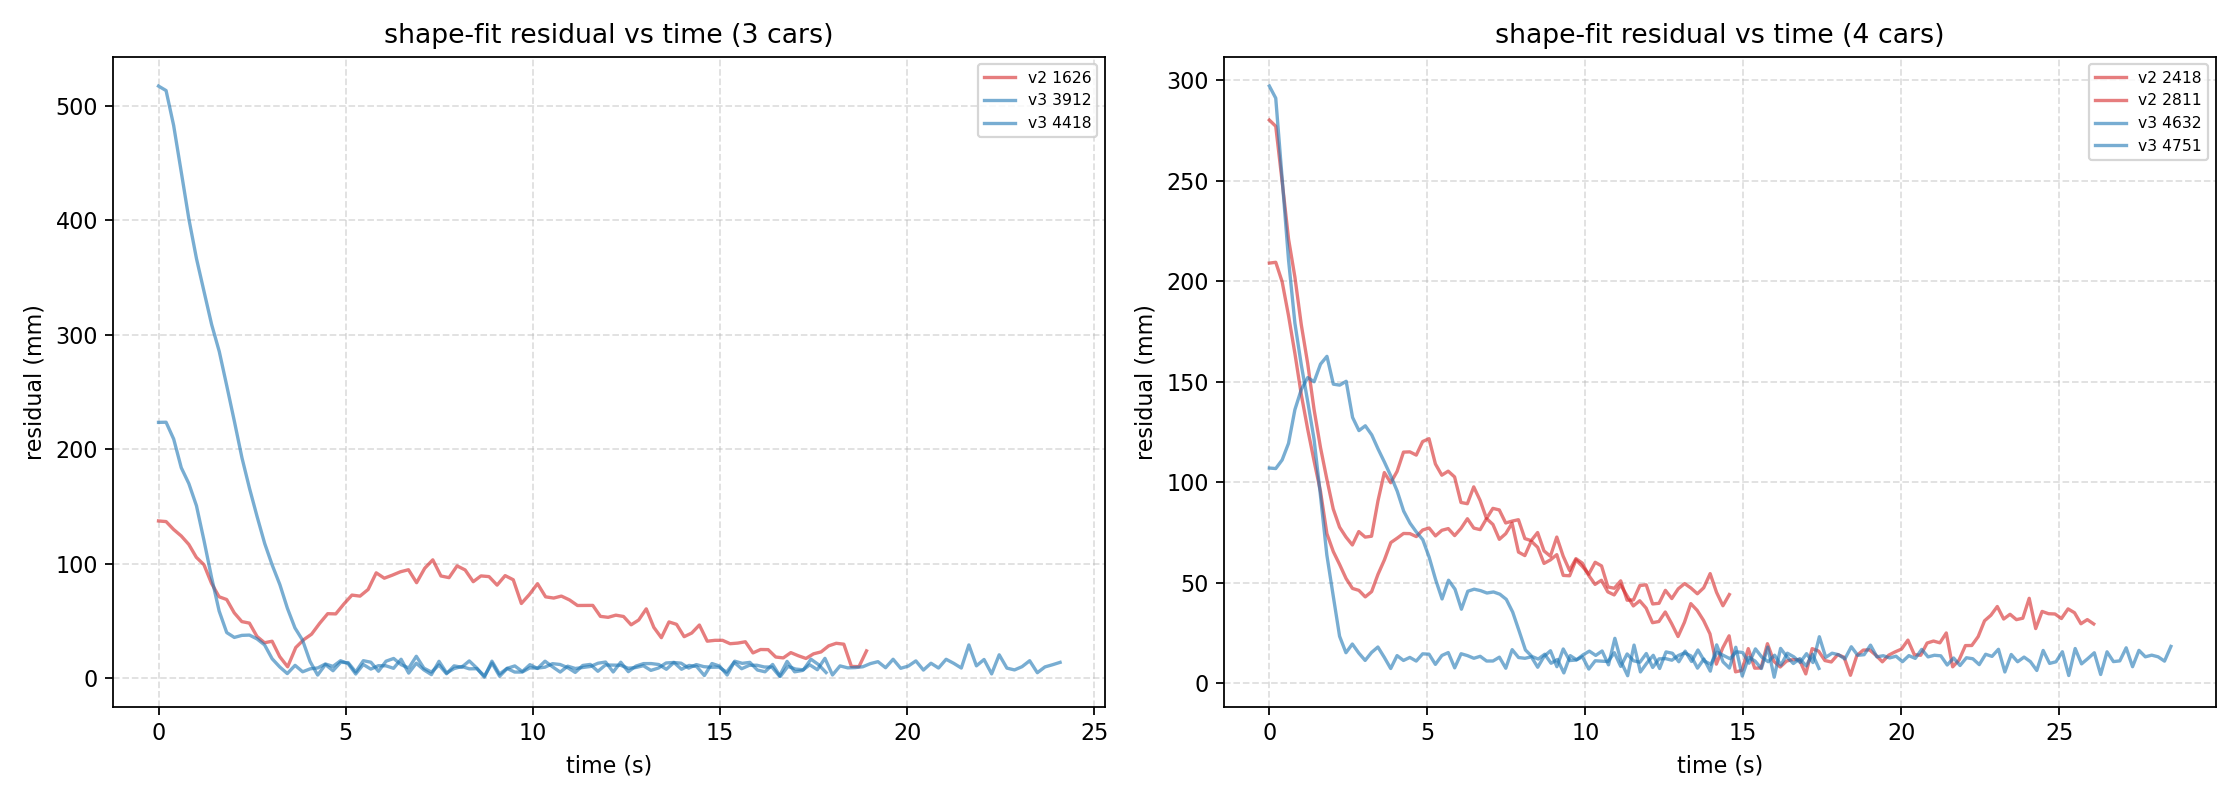
\includegraphics[width=\linewidth]{analysis/figs/fig5_v2v3.png}
\caption{形状拟合残差时间序列（版本中立口径，吸收平移/旋转/尺度）：
v3（蓝）快速收敛到约 10\,mm 量级；v2（红）停在 30--50\,mm 且 3 车组
后期缓慢爬升（爬行态）。}
\label{fig:v2v3}
\end{figure}

\begin{table}[H]
\centering\small
\caption{最终收敛对比（机动段末 5\,s；\file{results/fig5\_v2v3.json}）}
\label{tab:v2v3}
\begin{tabular}{llccc}
\toprule
规模 & 版本 & 形状残差 (mm) & 拟合尺度 & 拟合旋转 \\
\midrule
3 车 & v2（\run{1626}） & $26.2\pm8.4$ & 1.304（自由） & $+1.0\degC$ \\
 & v3（\run{3912}/\run{4418}） & $\mathbf{9.6\pm4.0}$ / $\mathbf{12.0\pm5.2}$
 & 1.000 / 0.991（锁定） & $+0.1\degC$ / $-0.5\degC$ \\
\midrule
4 车 & v2（\run{2418}/\run{2811}） & $48.2\pm6.4$ / $29.2\pm8.1$ & 0.759 / 0.640（自由）
 & $+1.7\degC$ / $-0.7\degC$ \\
 & v3（\run{4632}/\run{4751}） & $\mathbf{11.5\pm4.3}$ / $\mathbf{12.3\pm3.8}$
 & 1.001 / 0.999（锁定） & $\approx0\degC$ \\
\bottomrule
\end{tabular}
\end{table}

同一巡航速度（0.10\,m/s）、同一批车、相似的初始条件：v3 的形状保真度为
v2 的 2--4 倍，且 v3 额外锁定尺度与朝向（v2 原理上给不出）。
两车情形无形状自由度，对比由 fig2 的尺度锁定承担。

\section{行进振荡：归因修正与治理闭环（09-07 实验）}

\subsection{初版归因与其证伪}

初版分析（fig~\ref{fig:osc}、\ref{fig:oscattr}）曾将振荡归因于
\texttt{min\_eff} 量化本身：巡航目标 0.10\,m/s 的原始指令（$\approx20$）
低于死区补偿阈值 35，被钉死 $\pm35$ 形成 bang-bang。09-07 的 A/B 实车
对照\textbf{证伪}了"量化是根因"：affine（死区逆，连续映射）去掉了量化
（指令占比钉死 81\%$\to$2\%），振荡却与基线同频（约 1.4\,Hz）同幅甚至更差
——振荡器是环路本身，量化只是波形的外衣。

\begin{table}[H]
\centering\small
\caption{09-07 死区策略 A/B 对照（\file{runs\_ab/}；指标为末 10\,s 机动段，
\file{results/fig9\_ab\_comparison.json}）}
\label{tab:ab}
\begin{tabular}{lcccc}
\toprule
组 & 换向率 (次/s/轮) & 速度波纹中位 & yaw 摆动中位 & 稳态边误差 (m) \\
\midrule
基线 lift & 1.7--1.9 & 49--51\% & $3.7\degC$--$10.0\degC$ & 0.0317 \\
affine（死区逆） & 2.4 & 49--61\% & $8.2\degC$--$12.7\degC$ & 0.0423（变差） \\
\textbf{pwm（未标定）} & \textbf{0.3--0.6} & 46\% & $1.9\degC$--$3.1\degC$ & \textbf{0.0171} \\
hdb（航向死区 0.035） & 2.5 & 66--68\% & $2.4\degC$--$2.8\degC$ & 0.0306 \\
ema（$\alpha=0.5$） & 2.5--2.8 & 59\% & $2.1\degC$--$3.1\degC$ & 0.0261 \\
all（affine$+$hdb$+$ema） & 3.0--3.1 & 55--62\% & $2.8\degC$--$4.4\degC$ & 0.0411（变差） \\
\bottomrule
\end{tabular}
\end{table}

\subsection{修正后的机理：连续不可达区与时间平均}

低速死区的真实形态（09-07 实测）：cmd$<25$ 静摩擦锁死；cmd$\approx35$ 的
\textbf{最低可持续速度}为 0.10--0.18\,m/s（逐车不同，标定见下节）。
巡航 0.10\,m/s 落在"连续推力物理不可达"区间：闭环要么用极限环自我平均
（lift/affine），要么用时间平均（PWM）。修正结论：
\textbf{振荡本体是"PI 速度环 $+$ 低速死区"的组合体，不是量化本身；
PWM 并非消灭死区，而是把"平均"从环路手里夺走、交给 5\,Hz 载波去做}，
车体的机械惯性（一阶低通）把载波滤成平稳推进，环路重新看到近似线性的
对象而安静下来（换向率塌缩 4--8 倍）。

\subsection{仿真佐证（\file{scripts/sim\_limit\_cycle.py}）}

一阶车体 $+$ 滞滑死区（释放 35/保持 15，$v(35)=0.175$）$+$ 滞后估计器
$+$ 实车同款 PI 的标量仿真给出与实车一致的三元组：
无死区 $\to$ 零振荡（死区是振荡的\textbf{必要条件}）；
lift 与 affine 同频振荡（affine 不是解）；
PWM $\to$ 换向归零。扫参另得两条：PI 增益全域内 lift/affine 极限环均在
（调 PI 不是解）；PWM 载波 4--10 拍（50\,Hz 下 5--12.5\,Hz）良好，
20 拍过慢。仿真幅度（4--6\%）低于实车（46--77\%），因逐轮不对称与
滞滑强度未被单标量模型覆盖——仿真用于机制判别，不用于幅度预测
（\file{results/sim\_limit\_cycle.json}，图 \file{figs/fig8\_sim\_limit\_cycle.png}）。

\subsection{逐车归一化：标定与最终效果}

逐车标定（\file{tools/calibrate\_car.py}，动捕自动测速）给出
car4：$v(35)=0.201$\,m/s、car5：$v(35)=0.283$\,m/s——同指令下增益差 41\%。
补偿器按 $\mathrm{duty}=(c\cdot\mathrm{calib}/100)/v_{on}$ 逐车归一化
占空比（\file{results/fig9\_ab\_comparison.json}）：

\begin{table}[H]
\centering\small
\caption{逐车 $v_{on}$ 归一化前后（同巡航速度配对；$\dagger$1344 末尾含一次
动捕 yaw 跳变事件（$\pm130\degC$，外部扰动），剔除后约 0.015--0.016\,m）}
\label{tab:von}
\begin{tabular}{llccccc}
\toprule
组 & $v_{on}$ & 边误差 (m) & car4 达成率 & car5 达成率 & 波纹中位 & yaw 摆中位 \\
\midrule
1225 $w{=}0.1$ & 无 & 0.0142 & 94\% & 92\% & 26/26\% & $2.5\degC$/$1.0\degC$ \\
1227 $w{=}0.1$ & 无 & 0.0130 & 84\% & 81\% & 26/30\% & $1.2\degC$/$1.2\degC$ \\
1234 $w{=}0.2$ & 无 & 0.0144 & 87\% & 90\% & 10/13\% & $1.1\degC$/$1.0\degC$ \\
1342 $w{=}0.1$ & 0.201/0.283 & \textbf{0.0116} & \textbf{100\%} & 97\% & 13/18\% & $1.3\degC$/$0.8\degC$ \\
1344 $w{=}0.2$ & 0.201/0.283 & 0.0171$^\dagger$ & 95\% & \textbf{100\%} & 9/13\% & $4.7\degC$/$0.7\degC$ \\
\bottomrule
\end{tabular}
\end{table}

归一化直接达成设计目标：速度跟踪的系统偏差（$-6\%$/$-19\%$）消除，
两车达成率进入 $\pm5\%$ 以内；$w{=}0.1$ 组边误差收敛到
\textbf{0.0116\,m（全部批次最好）}；波纹降至 9--18\%。
治理链闭环：死区策略（PWM）$\to$ 逐车增益归一（$v_{on}$）$\to$
航向微振抑制（hdb=0.03）。

\begin{figure}[H]
\centering
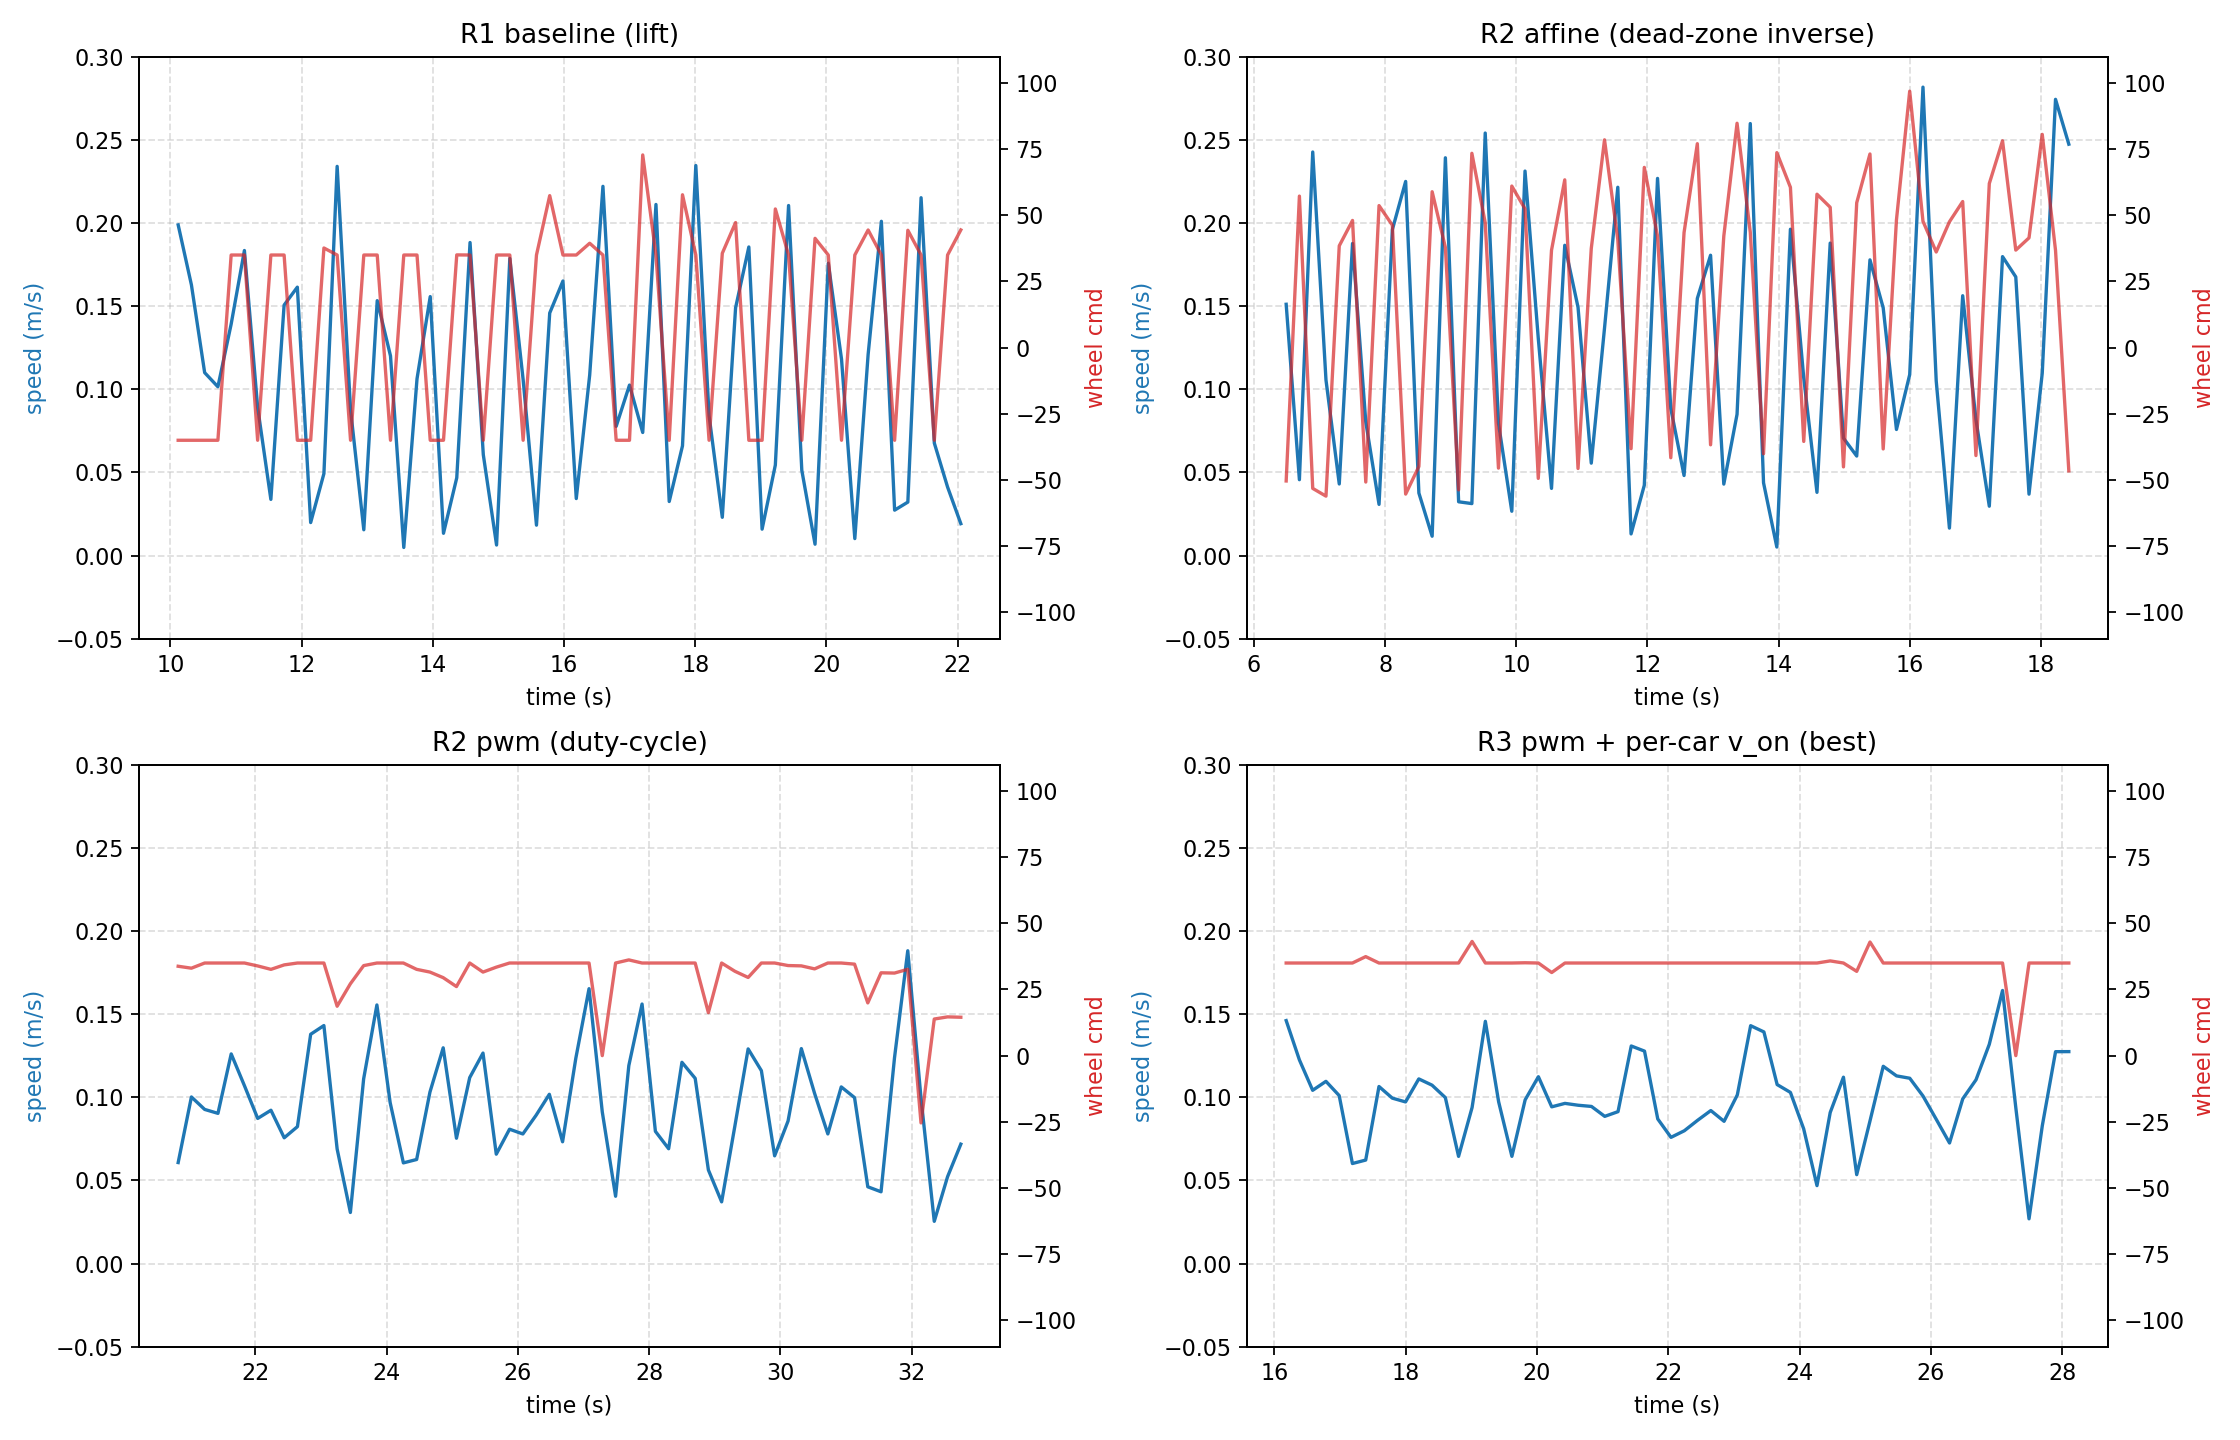
\includegraphics[width=\linewidth]{analysis/figs/fig10_waveforms.png}
\caption{振荡演进波形（同轴对比，蓝=实际车速，红=前轮指令）：
基线 lift 的 $\pm35$ bang-bang；affine 去量化后振荡依旧；PWM 的载波脉冲；
归一化 PWM（本轮最好）指令与速度双双走平。}
\label{fig:wave}
\end{figure}

\begin{figure}[H]
\centering
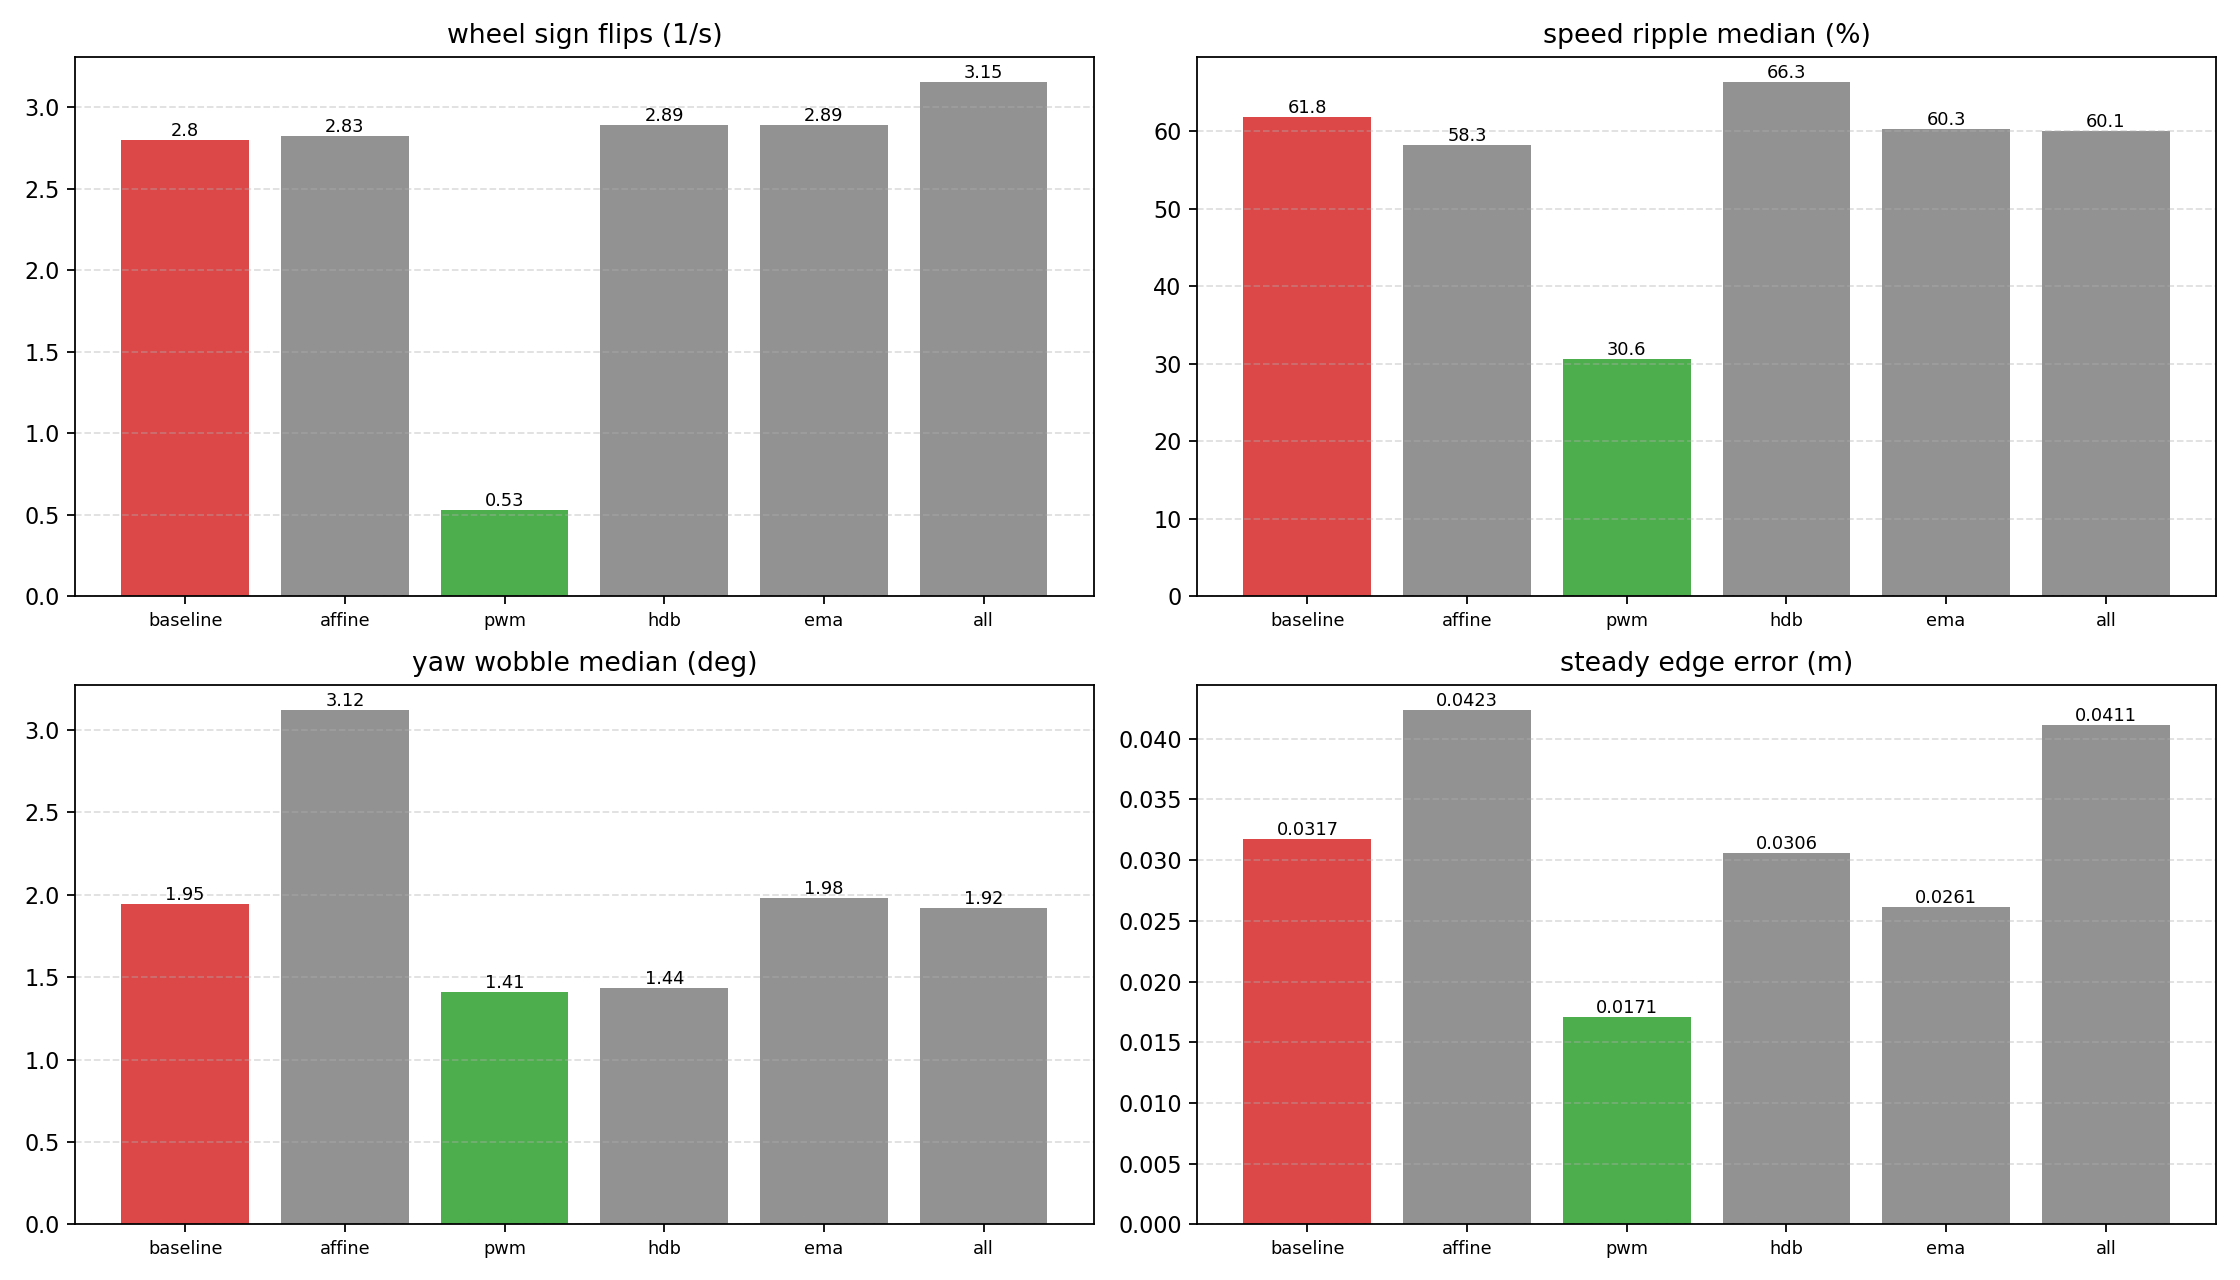
\includegraphics[width=\linewidth]{analysis/figs/fig11_ab_matrix.png}
\caption{09-07 死区策略 A/B 全指标矩阵（6 组 × 4 指标；绿=PWM 组）：
换向率、波纹、yaw 摆动、稳态边误差——PWM 全部最优或并列最优，
affine 全线持平或变差（\file{results/fig10\_12\_arc.json}）。}
\label{fig:abmatrix}
\end{figure}

\begin{figure}[H]
\centering
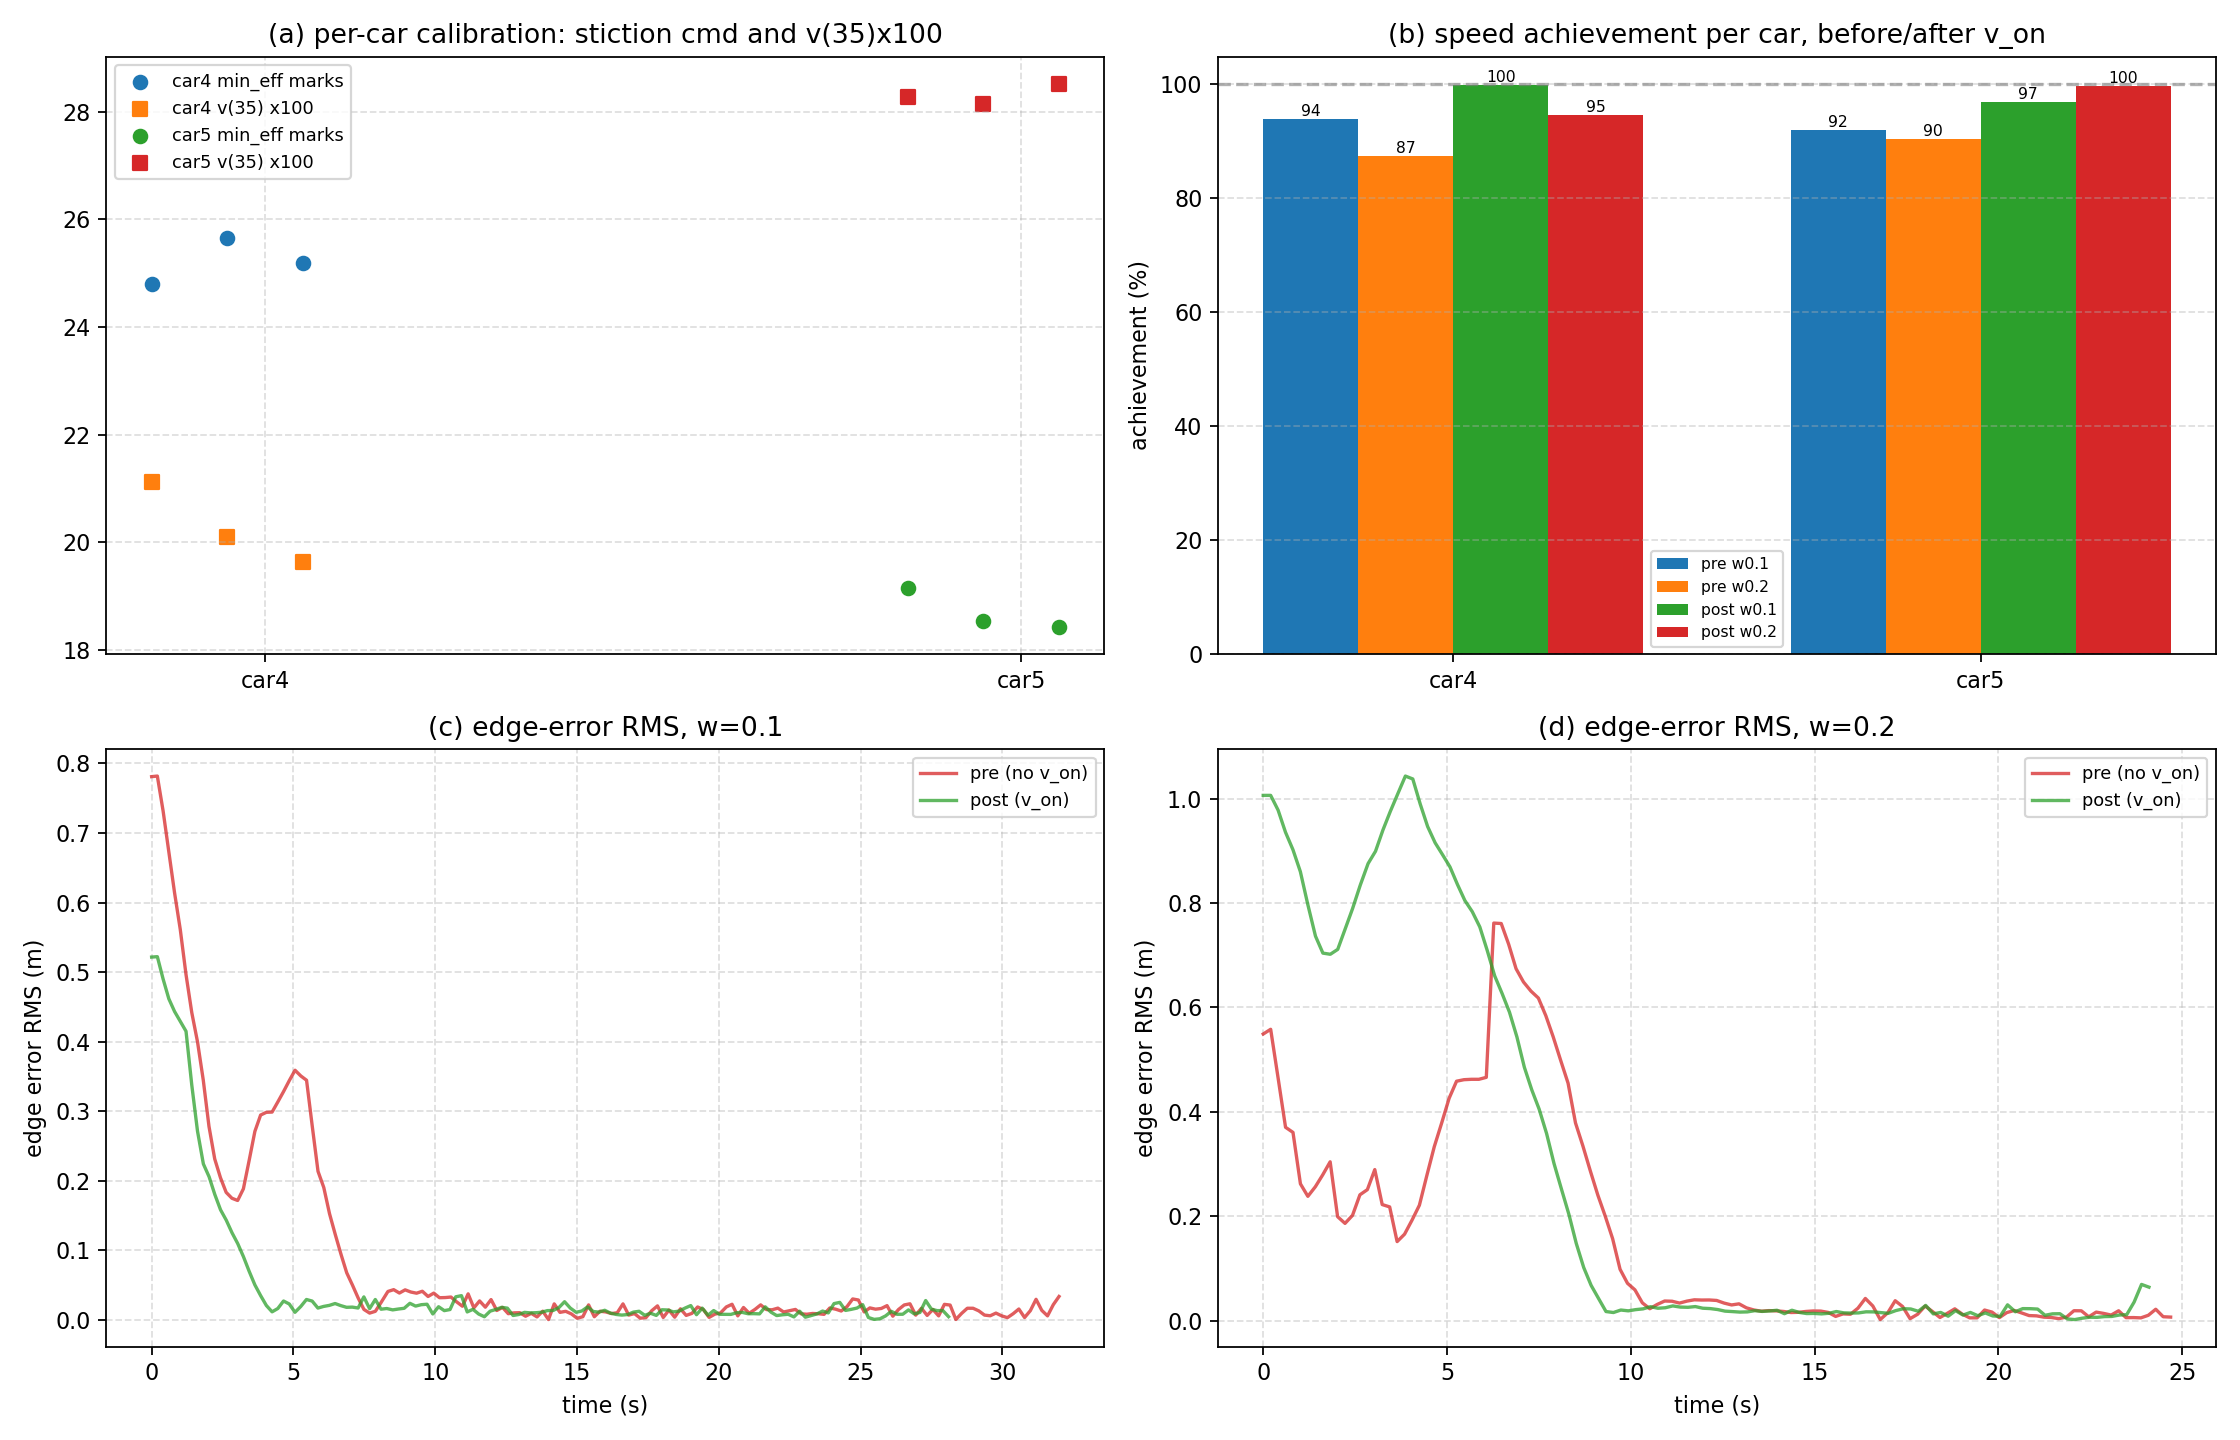
\includegraphics[width=\linewidth]{analysis/figs/fig12_von.png}
\caption{逐车 $v_{on}$ 归一化（\file{results/fig10\_12\_arc.json}）：
(a) 标定数据（静摩擦指令与 $v(35)$，car4/car5 增益差 41\%）；
(b) 归一化前后逐车速度达成率（95--100\% 命中）；
(c)(d) 两档巡航速度下边误差 RMS 曲线（前=红，后=绿）。}
\label{fig:von}
\end{figure}

\section{命题—指标—结果—证据总表}

\begin{table}[H]
\centering\small
\caption{命题验证总表}
\label{tab:budget}
\begin{tabular}{clp{4.2cm}p{4.2cm}l}
\toprule
\# & 命题 & 指标 & 实测结果 & 证据 \\
\midrule
P1 & 约束收敛 & 稳态边误差（米） & 0.022--0.030\,m（下限 0.019） & 图~\ref{fig:conv} \\
P2 & 尺度锁定 & 边距离 vs 期望 & 钉死，无漂移（v2 同期漂移） & 图~\ref{fig:scale} \\
P3 & 零空间解耦 & 质心速度达成率 & 90--99\%，误差衰减不受影响 & 图~\ref{fig:decouple} \\
P4 & 朝向锁定 & 拟合旋转 & $\approx0\degC$（v3）；尺度 $1.000\pm0.01$ & 表~\ref{tab:v2v3} \\
P5 & 泛化 & 2/3/4 车同栈 & 全部成立 & 图~\ref{fig:conv} \\
P6 & 起步设计 & 转向完成度 & 155--176$\degC$ 倒车 3\,s 内对准 & 图~\ref{fig:startup} \\
P7 & 振荡（已治理） & 低速死区 $\to$ PWM 时间平均 $+$ 逐车 $v_{on}$ 归一 $+$ 航向死区 & 换向 2.4$\to$0.1--0.6/s；边误差 0.0317$\to$0.0116\,m；达成率 82--94\%$\to$95--100\% & 表~\ref{tab:ab},\ref{tab:von} \\
\bottomrule
\end{tabular}
\end{table}

\section{不确定项}

\begin{enumerate}
  \item \run{v3\_two\_152637}（09-04）稳态 0.062\,m 为离群：后段存在一次
        未定位的漂移/扰动事件；\run{1344}（09-07）末尾动捕 yaw 跳变
        $\pm130\degC$（丢帧/标记遮挡），已标注并剔除解释，二者均非控制器行为。
  \item 尺度锁定的"长期不漂移"证据仅覆盖 17--38\,s；60\,s 级数据缺失。
  \item 中途变速/转向（多段 schedule）未做实验——任务驱动项的动态
        切换能力只有起步一段被验证。
  \item PWM 载波（5\,Hz 启停）对电机发热/机械磨损的影响未做长时评估；
        逐车 $v_{on}$ 目前只在 $w{=}0.1/0.2$\,m/s 两点验证。
  \item 全部实验为标量边权 $a_{ij}=1.0$：此时 null($L_A$) 恰为整体平移，
        矩阵加权带来的更丰富允许模态（尺度/预设形变）未涉及，
        属本批次的结构边界而非缺陷。
  \item 动捕原始二进制记录未解析（必要性低）；视频仅作时间戳核验，
        未抽帧配图。
\end{enumerate}

\section{对后续实验的建议}

\begin{enumerate}
  \item 跑 60\,s 长时运行确认尺度锁定长期性与 PWM 载波（5\,Hz）的
        电机耐受；$w{=}0.2$\,m/s 组补 1--2 轮（避开动捕干扰）钉死高速档结论。
  \item 做一轮中途变速（如 $t=10$\,s 时 $w$ 从 $(0.1,0)$ 切 $(0,0.1)$）
        验证任务动态切换。
  \item 扰动恢复实验（轻推一车）作为鲁棒性证据。
  \item 降载波幅值路径：在更低 ON 幅值（如 30/23，依逐车阈值）重测
        $v_{on}$ 并配对使用（\file{calibrated\_overrides.py} 的一致性
        规则已写入生成模块注释，勿跨级别混用）。
  \item 若论文强调 matrix-weighted 卖点：补一组非标量边权实验或仿真演示，
        展示扩展的允许运动模态。
\end{enumerate}

\appendix
\section{分析产物与复跑}

产物根目录 \file{report\_v3/analysis/}（全部为本次分析新建，未改动任何
原始记录）：

\begin{itemize}
  \item 脚本（\file{scripts/}）：\file{common.py}（v2/v3 双口径加载、
        相似变换拟合、机动段/稳态窗口）、\file{fig1\_fig2\_convergence\_scale.py}、
        \file{fig3\_fig4\_decoupling\_startup.py}、\file{fig5\_v2v3.py}、
        \file{fig6\_oscillation.py}、\file{fig7\_oscillation\_attribution.py}、
        \file{fig8\_sim\_limit\_cycle.py}（振荡仿真）、\file{fig9\_ab\_comparison.py}、
        \file{oscillation\_metrics.py}（单轮指标 CLI）。
        复跑：\texttt{cd report\_v3/analysis/scripts \&\& python <脚本>}。
  \item 图：\file{figs/fig1\_convergence.png}、\file{fig2\_scale\_lock.png}、
        \file{fig3\_decoupling.png}、\file{fig4\_startup.png}、
        \file{fig5\_v2v3.png}、\file{fig6\_oscillation.png}、
        \file{fig7\_oscillation\_attribution.png}、\file{fig8\_sim\_limit\_cycle.png}、
        \file{fig9\_ab\_comparison.png}、\file{fig10\_waveforms.png}、
        \file{fig11\_ab\_matrix.png}、\file{fig12\_von.png}。
  \item 数值结果：\file{results/fig1\_convergence.json}、
        \file{fig2\_scale\_lock.json}、\file{fig3\_decoupling.json}、
        \file{fig4\_startup.json}、\file{fig5\_v2v3.json}、
        \file{fig6\_oscillation.json}、\file{fig7\_oscillation\_attribution.json}、
        \file{sim\_limit\_cycle.json}、\file{fig9\_ab\_comparison.json}、
        \file{fig10\_12\_arc.json}。
  \item 数据说明与判读口径：\file{report\_v3/README.md}；振荡专题：
        \file{oscillation\_analysis.md}（初版归因）、
        \file{oscillation\_reanalysis.md}（09-07 修正版）。
\end{itemize}

\end{document}
